\chapter{Processi stocastici}
\label{ch:teoriasegnali-capitolo6}
Si considera un fenomeno aleatorio di cui si effettua una misura per un esperimento. L'evoluzione del segnale registrato non è predicibile a priori come in un segnale deterministico. Il segnale che viene effettivamente osservato si dice una realizzazione di un \textsc{processo stocastico}\index{processo stocastico}.

\begin{figure}[!ht]
	
	\begin{tikzpicture}
		\draw[-latex] (0,0) -- (8,0) node[right]{$t$};
		\draw[-latex] (0,0) -- (0,5);
		\draw [decorate, decoration={random,segment length=5pt,amplitude=20pt}] (0,1) -- (8,1) node [right] {$x_3(t)$} ;
		\draw [decorate, decoration={random,segment length=5pt,amplitude=20pt}] (0,2.5) -- (8,2.5) node [right] {$x_2(t)$};
		\draw [decorate, decoration={random,segment length=5pt,amplitude=20pt}] (0,4) -- (8,4) node [right] {$x_1(t)$};
		\draw (13,2.5) circle(2);
		\node at (14.8,4) {$\Omega$};
		\node (x1) at(13,3.8){};
		\node (x2) at(12,2.2){};
		\node (x3) at(13.5,1.2){};
		\fill (x1) circle(2pt) node[below]{$\omega_1$};
		\fill (x2) circle(2pt) node[below]{$\omega_2$};
		\fill (x3) circle(2pt) node[below]{$\omega_3$};
		\draw[-latex] (9.2,4) to[bend left](x1);
		\draw[-latex] (9.2,2.5) to[bend left](x2);
		\draw[-latex] (9.2,1) to[bend right](x3);
		\draw[dashed] (4,5)--(4,0)node[below]{$t_0$};
	\end{tikzpicture}
	\caption{Processo aleatorio}
\end{figure}

In altre parole un processo aleatorio mette in corrispondenza un particolare campione nello spazio di probabilità, $\omega_i$ in $\Omega=\{\omega_i\}$, con una sua particolare realizzazione $x_i(t)$ che ha la sua particolare evoluzione temporale. Tale corrispondenza è riassunta nella scrittura
\begin{equation}
	X(t;\omega_i)=x_i(t)
\end{equation}
In forma abbreviata, omettendo $\omega_i$ si indica con $X(t)$ il \textsc{processo aleatorio} per la generica realizzazione $x_i(t)$.
Una realizzazione del processo stocastico non è più aleatoria, a posteriori dell'osservazione essa è funzione deterministica del tempo.

Viceversa è possibile fissare un istante di tempo $t=t_0$ ed osservare il valore di tutte le realizzazioni del processo $X(t_0)$: i valori assunti dalle varie realizzazioni non sono predicibili a priori quindi rappresentano i risultati di una variabile aleatoria.

Un \textsc{processo aleatorio parametrico}\index{processo stocastico!parametrico} è un processo in cui il segnale nel tempo ha uno o più parametri descritti da una variabile aleatoria. Ad esempio
\[
	X(t;\omega)=\e{-A(\omega)t}\step(t)
\]
con $A(\omega)$ variabile aleatoria uniformemente distribuita nell'intervallo $[0,T]$.
Si può omettere l'indicazione di $\omega$
\[
	X(t)=\e{-A t}\step(t)\quad A\sim\text{unif.dist.}[0,T]
\]
Un ulteriore esempio è l'oscillatore reale a fase incerta
\[
	X(t)=A\sen{2\pi f_0 t+\phi}\quad \phi\sim\text{unif.dist.} [0,2\pi[
\]

\section{Caratterizzazione statistica di processi aleatori}
Per un fissato istante $t_0$, i valori che assumono tutte le realizzazioni di un processo $X(t)$ rappresentano una variabile aleatoria. Di questa variabile aleatoria si può definire una \textsc{funzione di distribuzione di probabilità del primo ordine}\index{variabile aleatoria!funzione distribuzione di probabilità!del primo ordine} che dipende da $t_0$:
\begin{equation}
	F_X(x;t_0)=P(X(t_0)\leq x)
\end{equation}

Per meglio caratterizzare un processo si può definire una \textsc{funzione di distribuzione di probabilità del secondo ordine o congiunta}\index{variabile aleatoria!funzione distribuzione di probabilità!del secondo ordine o congiunta} per una coppia di variabili aleatorie considerando due istanti di tempo differenti $t_1$ e $t_2$:
\begin{equation}
	F_X(x_1,x_2;t_1,t_2)=P(X(t_1)\leq x_1,X(t_2)\leq x_2)
\end{equation}

Per estensione una caratterizzazione completa di un processo stocastico richiede di determinare la \textsc{funzione di distribuzione di probabilità di ordine $n$}\index{variabile aleatoria!funzione distribuzione di probabilità!di ordine $n$}, fissati $n$ istanti di tempo e $n$ variabili aleatorie che si hanno estraendo i valori delle realizzazioni negli istanti $t_1,t_2,\dots,t_n$:
\begin{equation}
	F_X(x_1,\dots,x_n;t_1,\dots,t_n)=P(X(t_1)\leq x_1,\dots,X(t_n)\leq x_n)
\end{equation}

Dalle funzioni di distribuzioni di probabilità si ricava la \textsc{funzione densità di probabilità di ordine $n$}\index{variabile aleatoria!funzione densità di probabilità!di ordine $n$}:
\begin{equation}
	f_X(x_1,\dots,x_n;t_1,\dots,t_n)=\frac{\partial^n F_X(x_1,\dots,x_n;t_1,\dots,t_n)}{\partial x_1,\dots,\partial x_n}
\end{equation}

La conoscenza delle funzioni $f_X$ per ogni $n$ e per ogni $n$-pla di istanti di tempo caratterizza completamente il processo aleatorio. Una conoscenza completa è un'impresa praticamente impossibile. Nella maggioranza dei casi si cerca di determinare le distribuzioni e densità di probabilità del primo e secondo ordine e alcuni parametri statistici.

\section{Parametri statistici di primo ordine}
\index{processo stocastico!parametri statistici di primo ordine}
I parametri statistici valor medio, potenza e varianza permettono di determinare le caratteristiche principali di un processo aleatorio.

\subsection{Funzione valor medio}
La \textsc{funzione valor medio}\index{processo stocastico!parametri statistici di primo ordine!funzione valor medio} è definita come il valor medio della variabile aleatoria che si ottiene estraendo i valori delle realizzazioni nell'istante assegnato:
\begin{equation}
\label{eq:proc_valor_medio}
	\mu_X(t)=\E{X(t)}=\intinf{x f_X(x;t)}{x}
\end{equation}
La funzione valor medio è una statistica del primo ordine di $X(t)$ poiché il suo calcolo richiede la funzione densità di probabilità del primo ordine (funzione di una variabile aleatoria estratta dal processo e un istante di tempo).

\begin{esempio}
Si ha ad esempio il processo aleatorio parametrico
\[
	X(t)=a\cos{2\pi f_0 t+\Theta}\quad\Theta\sim\text{v.a.unif.} [0,\pi[
\]
Le funzioni campione del processo sono segnali cosinusoidali aventi medesima ampiezza e frequenza ma fase iniziale incerta. Per un fissato valore di $t$ si ha una variabile aleatoria $a\cos{2\pi f_0 t+\Theta}$ ottenuta come trasformazione della variabile aleatoria $\theta$.
Per il teorema del valor medio della variabile aleatoria
\begin{equation}
\label{eq:esempio_processo_non_stazionario_valor_medio}
	\begin{split}\mu_X(t)&=\E{X(t)}=\E{a\cos{2\pi f_0 t+\Theta}}=\intinf{ a\cos{2\pi f_0 t+\theta}f_\Theta(\theta)}{\theta}=\\
	&=\frac{a}{\pi}\intd{0}{\pi}{\cos{2\pi f_0 t+\theta}}{\theta}=\frac{a}{\pi}\bound{0}{\pi}{\sen{2\pi f_0 t+\theta}}=\\
	&=\frac{a}{\pi}\bound{0}{\pi}{\sen{2\pi f_0 t}\Cos\theta+\cos{2\pi f_0 t}\Sen\theta}=-\frac{2a}{\pi}\sen{2\pi f_0 t}
\end{split}
\end{equation}

Il valor medio è una funzione del tempo $t$.
\end{esempio}

\begin{esercizio}
Dato il processo aleatorio parametrico
\[
	X(t)=a\cos{2\pi f_0 t+\Theta}
\]
con $\Theta$ variabile uniforme in $[0,2\pi[$ mostrare che il valor medio $\mu_X(t)=0$.
\end{esercizio}

\subsection{Potenza media statistica istantanea}
La \textsc{potenza media}\index{processo stocastico!parametri statistici di primo ordine!potenza media} è una grandezza statistica del primo ordine che caratterizza un processo $X(t)$
\begin{equation}
	P_X(t)=\E{X^2(t)}=\intinf{x^2 f_X(x;t)}{x}
\end{equation}

\subsection{Funzione varianza}
La \textsc{funzione varianza}\index{processo stocastico!parametri statistici di primo ordine!funzione varianza} del processo aleatorio $X(t)$ è l'indice statistico del primo ordine
\begin{equation}
	\sigma^2_X(t)=\E{(X(t)-\mu_X(t))^2}=\intinf{(x-\mu_X)^2 f_X(x;t)}{x}
\end{equation}
La relazione di dipendenza tra varianza, funzione valor medio e potenza istantanea
\begin{equation}
	\sigma^2_X(t)=P_X(t)-\mu^2_X(t)
\end{equation}

\section{Parametri statistici di secondo ordine}
\index{processo stocastico!parametri statistici di secondo ordine}
Due parametri statistici del secondo ordine, fondamentali per lo studio dei processi stocastici, sono la \textsc{funzione autocorrelazione} e la \textsc{funzione autocovarianza}.

Dati due istanti di tempo arbitrari $t_1$ e $t_2$ è possibile estrarre dal processo due variabili aleatorie $X_1=X(t_1)$ e $X_2=X(t_2)$.

\subsection{Funzione di auto-correlazione}
La \textsc{funzione di autocorrelazione}\index{processo stocastico!parametri statistici di secondo ordine!funzione di autocorrelazione} misura la correlazione tra due variabili aleatorie estratte da uno stesso processo in due istanti di tempo $t_1$ e $t_2$:
\begin{equation}
\label{eq:proc_autocorrelazione}
	R_X(t_1,t_2)=\E{X(t_1)X(t_2)}=\intinf{\intinf{x_1 x_2 f_X(x_1,x_2;t_1,t_2)}{x_1}}{x_2}
\end{equation}

\subsection{Funzione di auto-covarianza}
Analogamente, la \textsc{funzione di auto-covarianza}\index{processo stocastico!parametri statistici di secondo ordine!funzione di autocovarianza} misura la covarianza di due variabili aleatorie estratte da uno stesso processo in due istanti di tempo $t_1$ e $t_2$:
\begin{equation}
\label{eq:proc_autocovarianza}
	\begin{split}
		C_X(t_1,t_2)&=\E{(X(t_1)-\mu_X(t_1)(X(t_2)-\mu_X(t_2)}=\\
		&=\intinf{\intinf{(x_1-\mu_X(t_1))(x_2-\mu_X(t_2))f_X(x_1,x_2;t_1,t_2)}{x_1}}{x_2}=\\
		&=R_X(t_1,t_2)-\mu_X(t_1)\mu_X(t_2)
	\end{split}
\end{equation}

\begin{esempio}
\label{es:oscillatore_non_stazionario}
Si calcoli l'autocorrelazione del processo aleatorio
\[
	X(t)=a\cos{2\pi f_0 t+\theta}\text{ con }\theta\text{ v.a. unif.dist. in }[0,\pi[
\]
Estraendo dal processo negli istanti $t_1$ e $t_2$ le variabili aleatorie
\[
	X(t_1)=a\cos{2\pi f_0 t_1+\theta}\quad X(t_2)=a\cos{2\pi f_0 t_2+\theta}
\]
e ricordando che $\Cos\alpha\Cos\beta=\frac{\cos{\alpha+\beta}+\cos{\alpha-\beta}}{2}$

\begin{equation}
\label{eq:autocorrelazione_oscillatore_non_stazionario}
	\begin{split}
		R_X(t_1,t_2)&=\E{X(t_1)X(t_2)}=\E{a\cos{2\pi f_0 t_1+\theta}a\cos{2\pi f_0 t_2+\theta}}=\\
		&=\frac{a^2}{2}\E{\cos{2\pi f_0(t_1+t_2)+2\theta}+\underbrace{\cos{2\pi f_0(t_1-t_2)}}_{\text{non dipende da $\theta$}}}=\\
		&=\frac{a^2}{2}\frac{1}{\pi}\intd{0}{\pi}{\cos{2\pi f_0(t_1+t_2)+2\theta}}{\theta}+\frac{a^2}{2}\cos{2\pi f_0(t_1-t_2)}=\\
		&=\frac{a^2}{2\pi}\bound{0}{\pi}{\frac{\sen{2\pi f_0(t_1+t_2)+2\theta}}{2}}+\frac{a^2}{2}\cos{2\pi f_0(t_1-t_2)}=\\
		&=\frac{a^2}{\pi}\bound{0}{\pi}{\frac{1}{2}\frac{\sen{2\pi f_0(t_1+t_2)}\cos{2\theta}}{2}+\frac{1}{2}\frac{\cos{2\pi f_0(t_1+t_2)}\sen{2\theta}}{2}}+\\
		&\quad+\frac{a^2}{2}\cos{2\pi f_0(t_1-t_2)}=\\
		&=\frac{a^2}{\pi}\underbrace{\left[\frac{1}{2}\frac{\sen{2\pi f_0(t_1+t_2)}}{2}-\frac{1}{2}\frac{\sen{2\pi f_0(t_1+t_2)}}{2}\right]}_{=0}+\frac{a^2}{2}\cos{2\pi f_0(t_1-t_2)}=\\
		&=\frac{a^2}{2}\cos{2\pi f_0(t_1-t_2)}
	\end{split}
\end{equation}
con $\theta\sim U([0,\pi[)$ si ha $R_X(t_1,t_2)$ che è funzione della differenza $t_1-t_2$, quindi di una sola variabile.
\end{esempio}
\begin{esempio}
\label{es:oscillatore_stazionario}
Si supponga di avere lo stesso processo aleatorio dell'esempio precedente ma con variabili aleatoria distribuita uniformemente in $[0,2\pi[$. Si voglia calcolare la funzione valor medio, la funzione di autocorrelazione e autocovarianza.
\[
	\mu_X(t)=\E{X(t)}=\intd{0}{2\pi}{\frac{1}{2\pi}a\cos{2\pi f_0 t+\theta}}{\theta}=0
\]
Essendo la funzione valor medio nulla allora
\begin{equation}
\label{eq:autocorrelazione_oscillatore_stazionario}
	\begin{split}
		C_X(t_1,t_2)&=R_X(t_1,t_2)=\E{X(t_1)X(t_2)}=\\
		&=\intd{0}{2\pi}{\frac{1}{2\pi}a\cos{2\pi f_0 t_1+\theta}a\cos{2\pi f_0 t_2+\theta}}{\theta}=\frac{a^2}{2}\cos{2\pi f_0(t_1-t_2)}
	\end{split}
\end{equation}
che è il medesimo risultato dell'esempio precedente.
\end{esempio}

\begin{esempio}
Si ha il processo aleatorio oscillatorio con ampiezza variabile uniformemente distribuita in $[0,1]$:
\[
	X(t)=A\cos{2\pi f_0 t}\text{ con }A\sim U([0,1])
\]
La funzione valor medio, come parametro del primo ordine funzione del tempo $t$:
\[
	\mu_X(t)=\E{X(t)}=\E{A\cos{2\pi f_0 t}}=\E{A}\cos{2\pi f_0 t}=\frac{1}{2}\cdot\cos{2\pi f_0 t}
\]
Il parametro di secondo ordine, la funzione di autocorrelazione, funzione di $t_1$ e $t_2$:
\[
	\begin{split}
		R_X(t_1,t_2)&=\E{X(t_1)X(t_2)}=\E{A\cos{2\pi f_0 t_1}A\cos{2\pi f_0 t_2}}=\\&=\E{A^2}\cos{2\pi f_0 t_1}\cos{2\pi f_0 t_2}=\frac{1}{3}\cos{2\pi f_0 t_1}\cos{2\pi f_0 t_2}
	\end{split}
\]
essendo $\E{A^2}=\intd{0}{1}{x^2}{x}=\frac{1}{3}$. In questo caso la funzione autocorrelazione è funzione delle due variabili $t_1$ e $t_2$, e non della differenza $t_1-t_2$.

La funzione autocovarianza, dai parametri precedenti, si valuta
\[
	\begin{split}
		C_X(t_1,t_2)&=R_X(t_1,t_2)-\mu_X(t_1)\mu_X(t_2)=\\
		&=\frac{1}{3}\cos{2\pi f_0 t_1}\cos{2\pi f_0 t_2}-\frac{1}{2}\cos{2\pi f_0 t}\cdot\frac{1}{2}\cos{2\pi f_0 t}=\\&=\frac{1}{12}\cos{2\pi f_0 t_1}\cos{2\pi f_0 t_2}
	\end{split}
\]
\end{esempio}

\section{Processo di Bernoulli e suoi derivati}
\index{processo aleatorio!di Bernoulli}
Si consideri il processo aleatorio tempo discreto di Bernoulli, le cui realizzazioni indipendenti assumono valori $I_n=\{0,1\}$ in istanti di tempo discreti indicati con $n\in\N$. I valori assunti si presentano con probabilità
\begin{equation}
	I_n=\begin{cases}
		0&p\\
		1&1-p
	\end{cases}
\end{equation}
La funzione valor medio vale
\begin{equation}
	\mu_I(n)=\E{I_n}=p\cdot 0+(1-p)\cdot 1=1-p
\end{equation}
Potenza e varianza valgono rispettivamente
\[
	\E{I^2_n}=p\cdot 0^2+(1-p)\cdot 1^2=1-p
\]
\begin{equation}
	\sigma^2_I=\E{I^2_n}-\Esp^2[I_n]=(1-p)-(1-p)^2=p(1-p)
\end{equation}
La funzione di autocorrelazione, essendo le realizzazioni indipendenti, vale
\begin{equation}
	R_I(n,m)=\E{I_n I_m}=\E{I_n}\E{I_m}=(1-p)^2
\end{equation}
Si possono definire processi che sono trasformazioni del processo di Bernoulli, ad esempio
\begin{equation}
	D_n=2I_n-1=\begin{cases}
		-1&p\\
		1&1-p
	\end{cases}
\end{equation}
La funzione valor medio vale
\begin{equation}
	\mu_D(n)=\E{D_n}=p\cdot (-1)+(1-p)\cdot 1=1-2p
\end{equation}
La varianza, calcolando il valore quadratico medio,
\[
	\E{D^2_n}=p\cdot (-1)^2+(1-p)\cdot (+1)^2=p+1-p=1
\]
\begin{equation}
	\sigma^2_D=\E{D^2_n}-\Esp^2[D_n]=1-(1-2p)^2=1-1+4p-4p^2=4p(1-p)
\end{equation}
La funzione di autocorrelazione, essendo le realizzazioni indipendenti:
\begin{equation}
	R_D(n,m)=\E{D_n D_m}=\E{D_n}\E{D_m}=(1-2p)^2
\end{equation}

\subsection{Random walk unidimensionale}
\index{processo aleatorio!random walk unidimensionale}
Dal processo precedente si deriva il processo \textsc{random walk unidimensionale}
\begin{equation}
	S_n=D_1+D_2+\dots+D_n
\end{equation}
La funzione valor medio vale
\begin{equation}
	\mu_S(n)=\E{S_n}=n\E{D_n}=n(1-2p)
\end{equation}
che dipende da $n$. Essendo i processi indipendenti la varianza è somma delle varianze
\begin{equation}
	\sigma^2_S(n)=\sum_{i=1}^{n}\sigma^2_{D_i}(n)=n\,4p(1-p)
\end{equation}
La funzione di autocorrelazione vale
\begin{equation}
	R_S(n,m)=\E{S_n S_m}=\E{\sum D_n \sum D_m}=\sum_{j=1}^{n}\sum_{i=1}^{m}\E{D_j D_i}=n m(1-2p)^2
\end{equation}
Nella doppia sommatoria precedente si ha $n\times m$ prodotti $\E{D_j}\E{D_i}$ di cui $n\cdot m-n$ $\E{D_j}\E{D_i}$ e $n$ $\E{D^2_i}=1$. 
%TODO:controllare appunti diversi

Il range di valori che può assumere il processo è variabile con $n$. $S_n$ con $n$ fissato può assumere valori compresi tra $[-n,n]$. La probabilità che k valori siano pari a $+1$ e $n-k$ valori siano pari a $-1$ è dato dalla formula di Bernoulli per la probabilità
\[
	P(S_n=k-(n-k)=2k-n)=\binom{n}{k}(1-p)^k p^{n-k}
\]

\subsection{Segnale telegrafico casuale}
\index{processo aleatorio!segnale telegrafico casuale}
Una variante del processo di Bernoulli è il \textsc{segnale telegrafico casuale}. Le realizzazioni del processo sono funzioni continue che assumono solo valori discreti pari a $-1$ e $1$ e cambiano stato secondo il modello degli eventi aleatori o arrivi di un processo di Poisson con intensità $\alpha$. Inoltre si suppone che lo stato iniziale sia equiprobabile: $P(X(0)=1)=P(X(0)=-1)=\frac{1}{2}$

\begin{figure}[!htb]
	\centering
	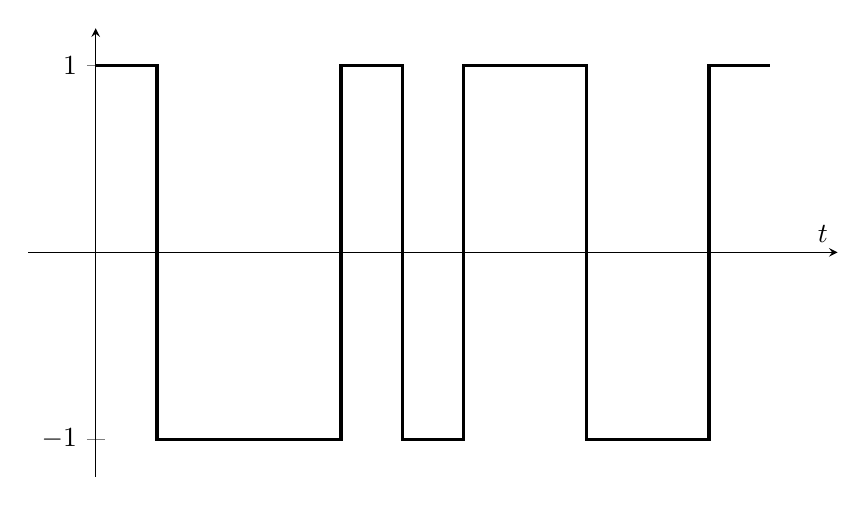
\begin{tikzpicture}
		\begin{axis}[axis lines=middle,no markers,enlargelimits,xscale=1.5,xtick={0},xlabel={$t$},ytick={-1,1}]
		\addplot [very thick]coordinates{(0,1)(1,1)(1,-1)(2,-1)(4,-1)(4,1)(5,1)(5,-1)(6,-1)(6,1)(8,1)(8,-1)(10,-1)(10,1)(11,1)};
		\end{axis}
	\end{tikzpicture}
\end{figure}

Si calcola la probabilità che ad un dato istante $t$ la singola realizzazione abbia uno dei due valori:
\begin{gather*}
	P(X(t)=1)=P(X(t)=1|X(0)=1)P(X(0)=1)+P(X(t)=1|X(0)=-1)P(X(0)=-1)
\end{gather*}
in cui la prima probabilità condizionata si ha per un numero di eventi pari di Poisson, mentre la seconda si ha per un numero di eventi dispari, ovvero
\begin{gather*}
\begin{cases}
	P(X(t)=1|X(0)=1) \Rightarrow \text{Probabilità di avere un numero pari di arrivi} \\
	P(X(t)=1|X(0)=-1) \Rightarrow \text{Probabilità di avere un numero dispari di arrivi}
\end{cases}
\end{gather*}
\begin{equation}
\begin{split}
	P(X(t)=1|X(0)=1)&=\sum_{k=0}^{+\infty}{\frac{(\alpha t)^{2k}}{(2k)!}\e{-\alpha t}}=\\
	&=\e{-\alpha t}\sum_{k=0}^{+\infty}{\frac{1}{2}\left[\frac{(\alpha t)^k}{k!}+\frac{(-\alpha t)^k}{k!}\right]}=\\
	&=\frac{\e{-\alpha t}}{2}(\e{\alpha t}+\e{-\alpha t})=\frac{1}{2}(1+\e{-2\alpha t})
\end{split}
\end{equation}
\begin{equation}
\begin{split}
	P(X(t)=1|X(0)=-1)&=\sum_{k=0}^{+\infty}{\frac{(\alpha t)^{2k+1}}{(2k+1)!}\e{-\alpha t}}=\\
	&=\e{-\alpha t}\sum_{k=0}^{+\infty}{\frac{1}{2}\left[\frac{(\alpha t)^k}{k!}-\frac{(-\alpha t)^k}{k!}\right]}=\\
	&=\frac{\e{-\alpha t}}{2}(\e{\alpha t}-\e{-\alpha t})=\frac{1}{2}(1-\e{-2\alpha t})
\end{split}
\end{equation}
da cui
\begin{equation}
	P(X(t)=1)=\frac{1}{2}\left[\frac{1}{2}(1+\e{-2\alpha t})+\frac{1}{2}(1-\e{-2\alpha t})\right]=\frac{1}{2}
\end{equation}
Analogamente si ha $P(X(t)=-1)=\frac{1}{2} \implies$ \textsc{processo senza memoria}\index{processo!senza memoria}.

Si calcola la funzione valor medio e la funzione varianza del processo:
\begin{equation}
	\mu_X(t)=\E{X(t)}=\frac{1}{2}\cdot(-1)+\frac{1}{2}\cdot(+1)=0
\end{equation}
\begin{equation}
	\sigma^2(t)=\E{X^2(t)}-\mu_X(t)^{2}=\frac{1}{2}\cdot(-1)^2+\frac{1}{2}\cdot(+1)^2-0=1
\end{equation}

La funzione di autocorrelazione e la funzione di autocovarianza, data la funzione valor medio, sono
\[
	C_X(t_1,t_2)=R_X(t_1,t_2)=\E{X(t_1)X(t_2)}
\]
il prodotto $X(t_1)X(t_2)$ può assumere solo due valori $+1$ o $-1$ a seconda del numero pari o dispari di arrivi nell'intervallo $[t_1,t_2[$, come si è visto con probabilità
\[
\begin{split}
	P(X(t_1)X(t_2)=1)&=\frac{1}{2}(1+\e{-2\alpha(t_2-t_1)})\\
	P(X(t_1)X(t_2)=-1)&=\frac{1}{2}(1-\e{-2\alpha(t_2-t_1)})
\end{split}
\]
pertanto si ha che
\begin{equation}
\begin{split}
	\E{X(t_1)X(t_2)}=\frac{1}{2}\left[(+1)(1+\e{-2\alpha(t_2-t_1)})+(-1)(1+\e{-2\alpha(t_2-t_1)})\right]=\e{-2\alpha(t_2-t_1)}
\end{split}
\end{equation}
ovvero funzione autocorrelazione e autovarianza dipendono dalla differenza dei due istanti di tempo generici e non dagli istanti stessi.

\section{Processi stazionari}
I \textsc{processi stazionari}\index{processo stazionario} hanno la notevole proprietà di mantenere costanti i parametri statistici determinati in $X(t)$ e in $X(t+\Delta t)$.

In generale si è visto che le funzioni densità di probabilità congiunta di ordine $n$ e i momenti di ordine $n$ dipendono dalla $n$-pla degli istanti di tempo $t_1,t_2,\dots,t_n$.

\subsection{Processo stazionario in senso stretto (SSS)}
Un processo aleatorio $X(t)$ è \textsc{stazionario in senso stretto (SSS)}\index{processo stazionario!in senso stretto} se le funzioni densità di probabilità congiunta di ogni ordine siano invarianti ad una traslazione rigida degli istanti di tempo, ovvero che per ogni ordine $n$
\begin{equation}
	\forall\Delta t\quad f_X(x_1,\dots,x_n;t_1,\dots,t_n)=f_X(x_1,\dots,x_n;t_1+\Delta t,\dots,t_n+\Delta t)
\end{equation}
Come corollario si ha che la stazionarietà di ordine $n$ implica la stazionarietà di ogni ordine inferiore.

Un processo stazionario in senso stretto ha quindi indici statistici che non distinguono il processo $X(t)$ dal processo $X(t+\Delta t)$.

Questo vuol dire ad esempio che la funzione densità di probabilità del primo ordine di un processo SSS è invariante rispetto al tempo $t$:
\[
	f_X(x;t)=f_X(x;t+\Delta t)\quad\forall\Delta t
\]

Di conseguenza tutte gli indici statistici del primo ordine non dipendono dal tempo $t$:
\[
	\mu_X(t)=\mu_X\quad \sigma^2_X(t)=\sigma^2_X
\]

Estraendo da un processo aleatorio stazionario in senso stretto di ordine 2 negli istanti di tempo $t_1$ e $t_2$ le variabili aleatorie $X(t_1)$ e $X(t_2)$ si ha la densità di probabilità congiunta
\[
	f_X(x_1,x_2;t_1,t_2)=f_X(x_1,x_2;t_1+\Delta t,t_2+\Delta t)\quad\forall\Delta t
\]
ovvero la funzione densità di probabilità congiunta non dipende dagli istanti di tempo separatamente ma dalla differenza dei due
\begin{equation}
	f_X(x_1,x_2;t_1,t_2)=f_X(x_1,x_2;t_1-t_2)
\end{equation}

Di conseguenza tutti gli indici statistici del secondo ordine, funzione autocorrelazione e autocovarianza, dipendono non dai singoli istanti di tempo ma dalla differenza $t_1-t_2$:
\[
	R_X(t_1,t_2)=R_X(t_1-t_2)\quad C_X(t_1,t_2)=C_X(t_1-t_2)
\]
inoltre dato che la stazionarità in senso stretto del secondo ordine implica la stazionarità in senso stretto di ordine 1 tutti i parametri statistici del primo ordine sono costanti.

In generale la densità di probabilità congiunta e tutte le statistiche di ordine $n$ di un processo stazionario in senso stretto dipenderanno solo dalle differenze $t_1-t_2, t_2-t_3, \dots, t_{n-1}-t_n$, che restano invariate in una traslazione rigida dei tempi.

\begin{nota}
	Per gli scopi ingegneristici la richiesta di stazionarietà in senso stretto è di difficile applicazione perché raramente le funzioni densità di probabilità di ogni ordine sono date in forma chiusa (notevole eccezione sono i processi gaussiani). Inoltre raramente si è interessati ad indici statistici di ordine superiore a due.
\end{nota}

\subsection{Processo stazionario in senso lato (SSL)}
Una definizione di stazionarietà meno restrittiva e più semplice da verificare: un processo aleatorio $X(t)$ è \textsc{stazionario in senso lato}\index{processo stazionario!in senso lato} se ha funzione valor medio nulla e funzione di autocorrelazione che dipende solo dalla differenza tra due generici istanti di tempo:
\begin{equation}
\label{eq:processo_stazionario_senso_lato}
	\begin{cases}
		\mu_X(t)=\mu_X\\
		R_X(t_1,t_2)=R_X(t_1-t_2)
	\end{cases}\implies \text{X(t) è un processo SSL}
\end{equation}
La funzione di autocorrelazione si può scrivere, ponendo $t_1=t$ e $t_2=t-\tau$, come
\begin{equation}
	R_X(t_1,t_2)=R_X(t,t-\tau)=\E{X(t)X(t-\tau)}=R_X(\tau)
\end{equation}
In tal caso anche la funzione autocovarianza dipende da $\tau=t_1-t_2$
\begin{equation}
	C_X(t_1,t_2)=R_X(t_1-t_2)-\mu^2_X=R_X(\tau)-\mu^2_X
\end{equation}

Non è richiesta alcuna proprietà di invarianza delle densità di probabilità che possono anche non essere conosciute in forma chiusa.
La stazionarietà di ordine 2 è condizione sufficiente per avere un processo SSL.
\begin{nota}
	La stazionarietà in senso lato non implica la stazionarietà in senso stretto.
\end{nota}
\begin{esempio}
Si è visto un esempio di processo aleatorio non stazionario definito dall'oscillatore
\[
	X(t)=a\cos{2\pi f_0 t+\theta}
\]
con fase $\theta$ variabile aleatoria a distribuzione uniforme in $[0,\pi[$
di cui si è calcolata la funzione valor medio (eq. \ref{eq:esempio_processo_non_stazionario_valor_medio})
\[
	\mu_X(t)=-\frac{2a}{\pi}\sen{2\pi f_0 t}
\]
Nonostante l'autocorrelazione (eq.\ref{eq:autocorrelazione_oscillatore_non_stazionario}) sia funzione di $t_1-t_2$, il processo non è stazionario dato che la funzione valor medio non è costante ma dipende dal tempo $t$.
\end{esempio}

\begin{esempio}
\label{es:oscillatore_stazionario_senso_lato}
Un esempio di processo aleatorio stazionario in senso lato è l'oscillatore
\[
	X(t)=a\cos{2\pi f_0 t+\theta}
\]
con fase $\theta$ variabile aleatoria a distribuzione uniforme in $[0,2\pi[$
che ha funzione valor medio funzione $\mu_X(t)=0$, quindi non dipende da $t$ e funzione di autocorrelazione (eq.\ref{eq:autocorrelazione_oscillatore_stazionario}) che dipende solo da $t_1-t_2$:
\[
	R_X(t_1,t_2)=\frac{a^2}{2}\cos{2\pi f_0(t_1-t_2)}
\]
\end{esempio}

\section{Processo telegrafico casuale: segnale dati}
\index{processo aleatorio!segnale dati}
Si supponga di avere un processo stocastico che modelli un segnale dati binario con frequenza di clock $\frac{1}{T}$ in modo da rappresentare la trasmissione di bit tra due sistemi.

Le realizzazioni sono funzioni $V(t)$ che possano assumere solo due valori discreti $+1$ e $-1$ e i cambi di stato avvengono in istanti di tempo multipli interi di un periodo $T$.
\begin{equation}
	V_n=\begin{cases}
		1&p=\frac{1}{2}\\
		-1&1-p=\frac{1}{2}
	\end{cases}
\end{equation}

I valori $V_n$ sono assunti in modo indipendente l'uno dall'altro e sono equiprobabili. La funzione si dice di \emph{sample and hold}: il segnale cambia di stato in istanti prefissati e mantiene costante il valore nell'intervallo di tempo tra transizioni successive $V(t)=V_n$ per $n T\leq t<(n+1)T$.
La funzione $V(t)$ è un treno di impulsi rettangolari scalati e traslati
\begin{equation}
\label{eq:segnale_dati}
	V(t)=\sum_{n=-\infty}^{+\infty}{V_n\rect{\frac{t-n T-\frac{T}{2}}{T}}}
\end{equation}

Dall'osservazione dei valori assunti e dall'equiprobabilità si desume la funzione densità di probabilità del primo ordine:
\begin{equation}
	f_V(v;t)=\frac{1}{2}\impulse(v-1)+\frac{1}{2}\impulse(v+1)
\end{equation}

La funzione densità di probabilità del primo ordine non dipende dal tempo quindi il processo è stazionario in senso stretto per il primo ordine. Infatti la funzione valor medio è costante
\begin{equation}
\label{eq:segnale_binario_media}
	\mu_V(t)=\intinf{v f_V(v;t)}{v}=\intinf{\frac{1}{2}v\impulse(v-1)+\frac{1}{2}v\impulse(v+1)}{v}=\frac{1}{2}-\frac{1}{2}=0
\end{equation}
La funzione valor medio può essere calcolata anche applicando l'operatore di aspettazione:
\begin{equation}
	\E{V(t)}=\sum_{n=-\infty}^{\infty}{\E{V_n}\rect{\frac{t-n T-\frac{T}{2}}{T}}}=0
\end{equation}
infatti $\E{V_n}=\frac{1}{2}\cdot(+1)+\frac{1}{2}\cdot(-1)=0$

Il calcolo della funzione di autocorrelazione, indice statistico del secondo ordine, avviene per due istanti di tempo generici $t_1$ e $t_2$. Come si può vedere in figura nel grafico di una realizzazione i due istanti di tempo possono assumere gli stessi valori $V(t_1)=V(t_2)=V_n$ all'interno di uno stesso intervallo di tempo, per cui
\begin{equation}
	R_V(t_1,t_2)=\E{V(t_1)V(t_2)}=\E{V(t_1)}\E{V(t_2)}=\E{V_n^2}=(+1)^2\cdot\frac{1}{2}+(-1)^2\cdot\frac{1}{2}=1
\end{equation}

In un'altra coppia di istanti di tempo è possibile trovarsi nella condizione $V(t'_1)\neq V(t'_2)$, ad esempio a cavallo di due intervalli in cui è avvenuto un cambio di stato, per i quali
\begin{equation}
	R_V(t'_1,t'_2)=\E{V(t'_1)V(t'_2)}=\E{V(t'_1)}\E{V(t'_2)}=\left(1\cdot\frac{1}{2}-1\cdot\frac{1}{2}\right)^2=0
\end{equation}
\begin{figure}[!h]
	\centering
	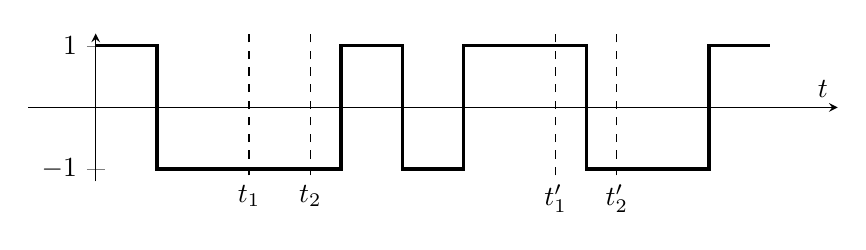
\begin{tikzpicture}
		\begin{axis}[axis lines=middle,no markers,enlargelimits,xscale=1.5,yscale=.33,xtick={0},xlabel={$t$},ytick={-1,1},clip=false]
		\addplot [very thick]coordinates {(0,1)(1,1)(1,-1)(2,-1)(4,-1)(4,1)(5,1)(5,-1)(6,-1)(6,1)(8,1)(8,-1)(10,-1)(10,1)(11,1)};
		\draw [dashed] (axis cs:2.5,-1.1) node[below]{$t_1$} -- (axis cs:2.5,1.2)
		(axis cs:3.5,-1.1) node[below]{$t_2$} -- (axis cs:3.5,1.2);
		\draw [dashed] (axis cs:7.5,-1.1) node[below]{$t'_1$} -- (axis cs:7.5,1.2)
		(axis cs:8.5,-1.1) node[below]{$t'_2$} -- (axis cs:8.5,1.2);
		\end{axis}
	\end{tikzpicture}
	\caption{Realizzazione di un processo dati binario}
	\label{fig:processo_dati_binario}
\end{figure}

Pertanto l'autocorrelazione dipende dai due istanti di tempo $t_1$ e $t_2$, questo implica che il processo non è stazionario in senso lato pur essendo stazionario in senso stretto per il primo ordine.

\section[Processo aleatorio con riferimento temporale aleatorio]{Processo aleatorio con riferimento temporale aleatorio: segnale eco radar}
\index{processo aleatorio!segnale eco radar}
Si modella il processo stocastico di un segnale di cui si conosce l'andamento ma il cui riferimento temporale è una variabile aleatoria $\theta$:
\begin{equation}
	X(t)=p(t-\theta)
\end{equation}

Ad esempio il segnale può essere un segnale periodico di periodo $T$: $p(t)=p(t+T)$. La variabile aleatoria uniformemente distribuita in $[0,T]$.

Si determinano le proprietà del processo. La funzione valor medio, calcolata sulla trasformata della variabile aleatoria $\theta$, che ha funzione densità di probabilità $f_\Theta(\theta)=\frac{1}{T}\rect{\frac{t-T/2}{T}}$:
\[
	\mu_X(t)=\E{p(t-\theta)}=\intd{0}{T}{p(t-\theta)\frac{1}{T}}{\theta}=\frac{1}{T}\intd{t}{t-T}{-p(\alpha)}{\alpha}=\frac{1}{T}\intd{t-T}{t}{p(\alpha)}{\alpha}
\]
dove si è posto $\alpha=t-\theta$, $\diff\alpha=-\diff\theta$, gli estremi di integrazione $\theta=0\to\alpha=t$, $\theta=T\to\alpha=t-T$.

L'integrale sulla funzione periodica su un intervallo di ampiezza $T$ non dipende dal valore $t$. Il valor medio statistico è pari al valor medio temporale della funzione $p(\alpha)$.

La funzione di autocorrelazione
\begin{align*}
	R_X(t_1,t_2)&=\E{p(t_1-\theta)p(t_2-\theta)}=\frac{1}{T}\intd{0}{T}{p(t_1-\theta)p(t_2-\theta)}{\theta}=\\
\intertext{cambio di variabile pongo $\alpha=t_1-\alpha$, $\diff\alpha=-\diff\theta$}
	&=\frac{1}{T}\intd{t_1}{t_1-T}{-p(\alpha)p(t_2-t_1+\alpha)}{\alpha}=\frac{1}{T}\intd{t_1-T}{t_1}{p(\alpha)p(t_2-t_1+\alpha)}{\alpha}=R_X(t_1-t_2)
\end{align*}

l'integranda è il prodotto di due termini periodici di periodo $T$, che è ancora di periodo $T$, quindi il suo integrale non dipende dal particolare istante iniziale di integrazione sul periodo. Pertanto la funzione autocorrelazione del processo $X(t)$ non dipende separatamente da $t_1$ e $t_2$ ma è funzione di $t_1-t_2$.

Essendo la funzione valor medio indipendente dal valor $t$ e la funzione autocorrelazione dipendente dal valore di $t_1-t_2$ il processo risulta stazionario in senso lato.

%\clearpage
\section{Proprietà funzione autocorrelazione processo SSL}
Proprietà della funzione di autocorrelazione di un processo stazionario in senso lato:
\begin{enumerate}
\item La funzione di autocorrelazione è pari
\[
	R_X(\tau)=R_X(-\tau)
\]
\begin{proof}[Dim.]
\[
	R_X(\tau)=\E{X(t)X(t-\tau)}=\E{X(t+\tau)X(t)}=R_X(-\tau)
\qedhere
\]
\end{proof}
\item Il valore assunto da $R_X(\tau)$ nell'origine è pari alla potenza statistica del processo
\[
	R_X(0)=P_X=\E{X^2(t)}
\]
\begin{nota}
	I processi aleatori SSL sono sempre segnali di potenza perché le varie realizzazioni che si estraggono da un processo non possono essere tutte infinitesime.
\end{nota}
\item La funzione autocorrelazione è massima in modulo nell'origine
\[
	R_X(0)\geq\abs{R_X(\tau)}
\]
\begin{proof}[Dim.]
\[
	\E{(X(t)\pm X(t-\tau))^2}\geq 0
\]
disuguaglianza sempre vera perché aspettazione di una quantità sempre positiva, sviluppando la relazione
\begin{gather*}
\E{X^2(t)}+\E{X^2(t-\tau)}\pm 2 \E{X(t)X(t-\tau)}\geq 0\\
2R_X(0)\pm 2R_X(\tau)\geq 0\\
R_X(0)\geq\pm R_X(\tau)\\
R_X(0)\geq\abs{R_X(\tau)}
\qedhere
\end{gather*}
\end{proof}
\item Se $R_X(\tau)$ non è periodica allora \begin{equation}
	\lim\limits_{\tau\to\infty}R_X(\tau)=\mu^2_X
\end{equation}
\begin{proof}[Dim.]
Per funzione di autocorrelazione che dipende solo dalla differenza dei tempi si ha che la funzione autocovarianza $C_X(\tau)=R_X(\tau)-\mu^2_X\xrightarrow{\tau\to\infty}0$ ovvero a crescere della distanza $\tau$ si hanno valori delle variabili aleatorie sempre meno correlati. La funzione di autocorrelazione pertanto $R_X(\tau)\xrightarrow{\tau\to\infty}\mu^2_X$.
\end{proof}
\end{enumerate}

\section[Processo aleatorio con riferimento temporale aleatorio]{Processo aleatorio: segnale dati binari}
Si considera nuovamente il segnale dati (eq.\ref{eq:segnale_dati}) con riferimento temporale non noto. Tale fenomeno si verifica ad esempio quando il ricevente riceve un segnale con un ritardo che dipende dalla distanza dal trasmittente. Un modello di questo processo con $\theta$ variabile aleatoria uniformemente distribuita in $[0,T]$, e valori $V_n$ indipendenti tra loro ed equiprobabili,
\[
	X(t)=V(t-\theta)=\sum_{n=-\infty}^{+\infty}V_n\rect{\frac{t-\theta-n T-T/2}{T}}
\]
Come abbiamo visto il segnale telegrafico casuale ha funzione valor medio costante e indenticamente nulla $\mu_X(t)=\mu_X=0$ (eq.\ref{eq:segnale_binario_media}).
Inoltre la funzione di autocorrelazione
\[
\begin{split}
	R_X(t_1,t_2)&=\E{X(t_1)X(t_2)}=\\
	&=\E{\sum_{n=-\infty}^{+\infty}\sum_{m=-\infty}^{+\infty}V_n V_m\rect{\frac{t_1-\theta-n T-\frac{T}{2}}{T}}\rect{\frac{t_2-\theta-m T-\frac{T}{2}}{T}}}=\\
\intertext{essendo $\E{V_nV_m}\neq 0$ solo se $n=m$, la doppia sommatoria si riduce ad un elemento}
	&=\sum_{n=-\infty}^{+\infty}\frac{1}{T}\intd{0}{T}{\rect{\frac{t_1-\theta-n T-T/2}{T}}\rect{\frac{t_2-\theta-m T-T/2}{T}}}{\theta}=\\
\intertext{cambio di variabili $t_1=t, t_2=t-\tau, \alpha=t-\theta-n T,\diff\alpha=-\diff\theta, \theta=0\to\alpha=t-nT, \theta=T\to t-(n+1)T$, inverto gli estremi per il segno di $-\diff\theta$}
	&=\frac{1}{T}\sum_{n=-\infty}^{+\infty}\intd{t-n T-T}{t-n T}{\rect{\frac{\alpha-T/2}{T}}\rect{\frac{\alpha-\tau-T/2}{T}}}{\alpha}=\\
\intertext{l'integranda non dipende da $n$, la sommatoria degli integrali su intervalli disgiunti $[n T-T,n T]$ può essere sostituita da un unico integrale}
	&=\frac{1}{T}\intd{-\infty}{+\infty}{\rect{\frac{\alpha-T/2}{T}}\rect{\frac{\alpha-\tau-T/2}{T}}}{\alpha}=\\
	&=\frac{1}{T}\rect{\frac{\tau-T/2}{T}}\ast\rect{\frac{-\tau-T/2}{T}}
\end{split}
\]
La funzione autocorrelazione dipende dalla sola variabile $\tau$ e rappresenta una correlazione deterministica convoluzione di due funzioni rettangolo che è pari ad una funzione triangolare.
Il segnale dati binario con ritardo casuale, pertanto, è un processo stazionario in senso lato.

\section{Significato funzione autocorrelazione processo SSL}
Presi due processi stocastici stazionari in senso lato $X(t)$ e $Y(t)$, dotati degli stessi parametri statistici del primo ordine (funzione valor medio, funzione potenza, funzione varianza), ad esempio con valor medio $\mu_X(t)=\mu_Y(t)=\text{costante}$. Per poter distinguere statisticamente i segnali si analizzano i parametri statistici del secondo ordine (funzione autocorrelazione, funzione autocovarianza).

Supponendo che $R_X(\tau)\neq R_Y(\tau)$ ho modo di distinguere i processi.
In particolare quello che si osserva per istanti di tempo distanti $\tau$ è una diversa velocità di variazione: infatti uno dei due segnali assomiglierà di più a se stesso (autocorrelazione maggiore), ovvero le variazioni delle realizzazioni sono più lente e quindi più somiglianti tra loro.

\section{Filtraggio processo aleatorio}
\index{processo aleatorio!filtraggio}
La teoria dei processi stocastici modella fenomeni reali descrivibili da grandezze fisiche che variano nel tempo in modo non predicibile a priori. Essendo le grandezze fisiche manipolabili ha senso chiedersi cosa significa filtrare un processo aleatorio attraverso un sistema.

In particolare per sistemi lineari tempo-invarianti si avrà che un segnale $x(t)$ in ingresso al sistema sarà convoluto con la risposta all'impulso del sistema per avere in uscita un segnale $y(t)=x(t)\ast h(t)$.

Nei processi aleatori avremo usualmente un segnale deterministico noto a cui è sovrapposto un segnale di disturbo o rumore che è modellato dal processo aleatorio a valor medio nullo. Compito dell'ingegnere è progettare filtri che eliminino, almeno in parte, la componente rumorosa dalle realizzazioni del processo.

\begin{figure}[!h]
	\centering
	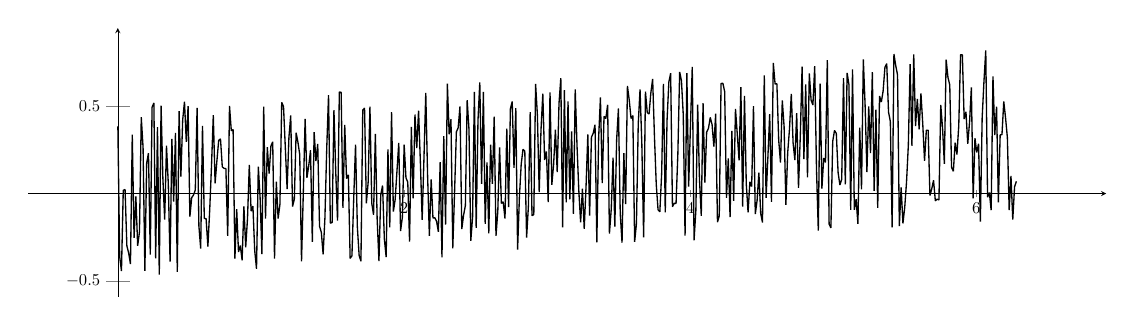
\begin{tikzpicture}[scale=.6]
		\begin{axis}[axis lines=middle,no markers,enlargelimits,xscale=3.33,line join=bevel]
		\addplot [thick,domain=0:6.28,samples=500] {sin(pi*x+0.5)+.5*rand};
		\end{axis}
	\end{tikzpicture}
	\caption{Esempio di segnale deterministico affetto da rumore}
\end{figure}

Per ogni realizzazione $x(t;\omega)$ del processo $X(t)$ dello spazio campione $\Omega$ si otterrà in uscita dal sistema filtro una funzione $y(t)=x(t;\omega)\ast h(t)$. L'insieme dei segnali di uscita costituisce un nuovo processo aleatorio, $Y(t)$ che indichiamo con
\begin{equation}
	Y(t)=X(t)\ast h(t)
\end{equation}

\begin{figure}[!h]
	\centering
	\begin{tikzpicture}[node distance=3cm]
		\node [block] (system) at (0,0) {$h(t)$};
		\node [left of=system](input) {};
		\node [right of=system] (output) {};
		\draw [-latex] (input) -- (system) node[pos=.5,above]{$X(t)$};
		\draw [-latex] (system) -- (output) node[pos=.5,above]{$Y(t)$};
	\end{tikzpicture}
	\caption{Filtraggio del processo $X(t)$}
\end{figure}

Generalmente il problema di determinare la funzione densità di probabilità congiunta di qualunque ordine per il processo d'uscita, ammesso che sia nota quella del processo di ingresso, è insolubile.

Si determina allora la relazione dei parametri statistici di primo e secondo ordine in ingresso, almeno la funzione valor medio e la funzione autocorrelazione di $X(t)$, e i corrispondenti dell'uscita.

\textbf{Funzione valor medio del processo in uscita $Y(t)$}
\begin{equation}
\begin{split}
	\mu_Y(t)&=\E{Y(t)}=\E{X(t)\ast h(t)}=\E{\intinf{h(\tau)X(t-\tau)}{\tau}}=\\
	&=\intinf{\E{h(\tau)X(t-\tau)}}{\tau}=\intinf{h(\tau)\E{X(t-\tau)}}{\tau}=\\
	&=\intinf{h(\tau)\mu_X(t-\tau)}{\tau}=\\
	&=\mu_X(t)\ast h(t)
\end{split}
\end{equation}
Il risultato $\mu_Y(t)=\mu_Y(t)\ast h(t)$ è notevole: la funzione valor medio in uscita si ottiene come convoluzione della funzione valor medio in ingresso con la risposta all'impulso del sistema. Pertanto un sistema con in ingresso un segnale deterministico a cui si somma un processo stocastico a valor medio nullo, per la linearità del sistema, darà in uscita un processo somma di una componente deterministica e di una componente statistica che avrà ancora valor medio nullo. Il filtraggio ottimo elimina la componente statistica e preserva la componente deterministica.
\begin{equation}
	\underset{\text{proc.aleat.}}{X(t)} = \underset{\text{proc.aleat. a media nulla}}{X_0(t)} + \underset{\text{segn.determ.}}{\mu_x(t)}
\end{equation}

\textbf{Funzione di autocorrelazione del processo in uscita $Y(t)$}
\begin{equation}
\begin{split}
	R_Y(t_1,t_2)&=\E{Y(t_1)Y(t_2)}=\E{(X(t_1)\ast h(t_1))\cdot(X(t_2)\ast h(t_2))}=\\
	&=\E{\intinf{\intinf{X(\alpha)h(t_1-\alpha)X(\beta)h(t_2-\beta)}{\alpha}}{\beta}}=\\
	&=\intinf{\intinf{h(t_1-\alpha)h(t_2-\beta)\E{X(\alpha)X(\beta)}}{\alpha}}{\beta}=\\
	&=\intinf{\intinf{h(t_1-\alpha)h(t_2-\beta)R_X(\alpha,\beta)}{\alpha}}{\beta}=\\
	&=R_X(t_1,t_2)\ast h(t_1)\ast h(t_2)
\end{split}
\end{equation}

\section{Filtraggio processo stazionario in senso lato}
\label{sec:filtraggio_processo_SSL}
Si ha in ingresso al filtro un processo stazionario in senso lato, che ha funzione valor medio costante e funzione di autocorrelazione dipendente da $\tau=t_1-t_2$ (eq.\ref{eq:processo_stazionario_senso_lato}).

\textbf{Funzione valor medio del processo in uscita $Y(t)$ quando $X(t)$ è SSL}
\begin{equation}
	\mu_Y(t)=\mu_X(t)\ast h(t)=\intinf{h(\tau)\mu_X(t-\tau)}{\tau}=\mu_X\intinf{h(\tau)}{\tau}=\mu_X\cdot \restrict{H(f)}{f=0}=\text{cost}
\end{equation}
dove $H(0)$ è il valore della trasformata di Fourier della risposta all'impulso nell'origine, e la funzione valor medio in uscita assume valore costante.

\textbf{Funzione di autocorrelazione del processo in uscita $Y(t)$ quando $X(t)$ è SSL}
\begin{align*}
	R_Y(t,t-\tau)&=\E{Y(t)Y(t-\tau)}=\E{(X(t)\ast h(t))(X(t-\tau)\ast h(t-\tau))}=\\&=\E{\intinf{\intinf{h(\alpha)X(t-\alpha)h(\beta)X(t-\tau-\beta)}{\alpha}}{\beta}}=\\&=\intinf{\intinf{h(\alpha)h(\beta)\E{X(t-\alpha)X(t-\tau-\beta)}}{\alpha}}{\beta}=\\&=\intinf{\intinf{h(\alpha)h(\beta)R_X(\tau+\beta-\alpha)}{\alpha}}{\beta}=\\
	\intertext{si può osservare che la funzione di autocorrelazione non dipende da $t$ ma solo da $\tau$ pertanto filtrando un processo stazionario si ottiene un processo stazionario,}
	&=\intinf{h(\beta)\underbrace{\left[\intinf{R_X(\tau+\beta-\alpha)h(\alpha)}{\alpha}\right]}_{R_X(\tau+\beta)\ast h(\tau+\beta)=g(\tau+\beta)}}{\beta}=\\
	&=\intinf{h(\beta)g(\tau+\beta)}{\beta}=\intinf{h(-z)g(\tau-z)}{z}=g(\tau)\ast h(-\tau)
\end{align*}

Si ottiene quindi
\begin{equation}
	R_Y(\tau)=R_X(\tau)\ast h(\tau)\ast h(-\tau)=R_X(\tau)\ast R_h(\tau)
\end{equation}
dove la convoluzione del segnale $h(\tau)\ast h(-\tau)$ è l'autocorrelazione del segnale deterministico risposta all'impulso.

Quando un processo stazionario in senso lato in ingresso ad un sistema lineare tempo invariante viene filtrato in uscita si ottiene un processo stazionario in senso lato.

Il filtraggio di un processo aleatorio $X(t)$ ha quindi due casi per cui la funzione valor medio e la funzione di autocorrelazione del processo in uscita sono legate a quelle del processo in ingresso.

\begin{table}[!h]
	\centering
	\begin{tabular}{c|c}
%		\toprule
			\multicolumn{2}{c}{$Y(y)=X(t)\ast h(t)$}\\
		\midrule
			caso $X(t)$ generico & caso $X(t)$ SSL\\
			$\begin{cases}
			\mu_Y(t)=\mu_X(t)\ast h(t)\\R_Y(t_1,t_2)=R_X(t_1,t_2)\ast h(t_1)\ast h(t_2)
			\end{cases}$ & $\begin{cases}
			\mu_Y(t)=\mu_X\cdot H(0)\\R_Y(\tau)=R_X(\tau)\ast R_h(\tau)
			\end{cases}$\\
%		\bottomrule
	\end{tabular}
\end{table}

